% Сборка из корня проекта:
% latexmk -xelatex -outdir=build/report 'output/pdf/Диниц отчёт.tex'
% Иллюстрации результатов берутся из results/ в корне проекта.
\documentclass[14pt,a4paper]{extarticle}

\usepackage[fontsize=14pt]{fontsize}
\usepackage[top=2cm,bottom=2cm,left=3cm,right=1.5cm]{geometry}
\usepackage{fontspec}
\usepackage{polyglossia}
\setdefaultlanguage{russian}
\setotherlanguage{english}
\IfFontExistsTF{Times New Roman}
  {\setmainfont{Times New Roman}}
  {\setmainfont{Tinos}}
\setmonofont{DejaVu Sans Mono}

\usepackage{amsmath}
\usepackage{setspace}
\usepackage{titlesec}
\usepackage{graphicx}
\usepackage{caption}
\usepackage{booktabs}
\usepackage{siunitx}
\usepackage{tikz}
\usetikzlibrary{arrows.meta,positioning}
\usepackage[unicode,hidelinks]{hyperref}

\makeatletter
\newcommand{\reportfontsize}[1]{\fontsize{#1}{\f@baselineskip}\selectfont}
\renewcommand{\l@section}[2]{%
  \begingroup
    \let\numberline\@gobble
    \@dottedtocline{1}{1.25cm}{0pt}{#1}{#2}%
  \endgroup
}
\renewcommand{\l@subsection}{\@dottedtocline{2}{1.85cm}{2.2em}}
\renewcommand{\@dotsep}{0.5}
\renewcommand{\@biblabel}[1]{#1.}
\makeatother

\hypersetup{
  pdftitle={Эмпирический анализ алгоритма Диница},
  pdfauthor={Михеев Григорий Дмитриевич},
  pdflang={ru-RU}
}
\graphicspath{{results/}{../../results/}}
\DeclareCaptionFont{report}{\reportfontsize{12pt}}
\captionsetup{font={singlespacing,report},labelsep=period,hypcap=false}
\newcommand{\reportCaptionNames}{\renewcommand{\figurename}{Рис.}\renewcommand{\tablename}{Таблица}}
\titleformat{\section}{\normalfont\centering\reportfontsize{18pt}\bfseries}{\thesection.}{0.5em}{}
\titleformat{\subsection}{\normalfont\centering\reportfontsize{16pt}\bfseries}{\thesubsection.}{0.5em}{}
\titlespacing*{\section}{0pt}{0.8em}{0.35em}
\titlespacing*{\subsection}{0pt}{0.6em}{0.35em}
\sisetup{output-decimal-marker={,},group-separator={\,},group-minimum-digits=4}
\setlength{\parindent}{1.25cm}
\setlength{\parskip}{0pt}
\setlength{\emergencystretch}{1em}
\onehalfspacing

\newcommand{\family}[1]{\texttt{#1}}
\newenvironment{resulttable}[2]{%
  \par\noindent\begin{minipage}{\linewidth}\centering
  \captionof{table}{#1}\label{#2}
  \singlespacing
  \reportfontsize{12pt}
  \setlength{\tabcolsep}{8pt}
  \begin{tabular}{@{}rrrrrrr@{}}
  \toprule
  $V$ & $E$ & $\bar C$ & $s$ & $\bar C/V$ & $\bar C/(V^2 E)$ & Рост\\
  \midrule
}{%
  \bottomrule
  \end{tabular}
  \end{minipage}\par\smallskip
}
\newcommand{\resultrow}[7]{%
  #1 & #2 & \num{#3} & \num{#4} & \num{#5} & \num{#6} & #7\\
}

\begin{document}
\reportCaptionNames

\begin{titlepage}
\thispagestyle{empty}
\centering
{\reportfontsize{12pt}
САНКТ-ПЕТЕРБУРГСКИЙ ГОСУДАРСТВЕННЫЙ УНИВЕРСИТЕТ\par}

\vspace{30pt}
{\reportfontsize{18pt}\bfseries Михеев Григорий Дмитриевич\par}

\vspace{37pt}
{\reportfontsize{18pt}\bfseries
Отчёт по индивидуальному заданию\\
учебной дисциплины\\
Алгоритмы и анализ сложности\par}

\vspace{50pt}
{\reportfontsize{18pt}\bfseries
Эмпирический анализ алгоритма Диница\\
для нахождения максимального потока\par}

\vspace{6pt}
Направление 02.03.02 «Фундаментальная информатика и информационные технологии»\par
Основная образовательная программа СВ.5003.2023 «Программирование и информационные технологии»\par

\vspace{48pt}
{\raggedright
Преподаватель,\\
кандидат физ.-мат. наук,\\
доцент\hfill Никифоров К.~А.\par}

\vspace{48pt}
Санкт-Петербург\\
2026
\end{titlepage}

\setcounter{page}{2}
\tableofcontents
\clearpage

\section{Введение и постановка задачи}

Цель работы --- выяснить, как структура сети влияет на число проверок дуг в алгоритме Диница при одинаковом числе вершин и дуг. Алгоритм опубликован Б. А.~Диницем в 1970 году~\cite{dinic}.

В ориентированной сети заданы исток $s$, сток $t$ и пропускная способность каждой дуги. Поток по дуге ограничен её пропускной способностью. Во внутренней вершине суммарный входящий поток равен исходящему. Требуется найти наибольший поток из $s$ в $t$. Задача используется, например, при планировании перевозок и поиске паросочетаний~\cite{sedgewick}.

\section{Краткое описание алгоритма}

Остаточная сеть показывает, какие изменения потока ещё возможны. Прямая остаточная дуга хранит свободную ёмкость. Обратная позволяет отменить часть ранее отправленного потока. В начале фазы BFS присваивает достижимым вершинам уровни по расстоянию от истока в остаточной сети. DFS ищет пути по дугам, которые ведут на следующий уровень, и отправляет вдоль найденного пути минимум его остаточных ёмкостей. Фаза заканчивается, когда все такие пути заблокированы~\cite{dinic,williamson}.

В примере на рис.~\ref{fig:network} первая фаза отправляет 2 единицы по пути $s \to a \to t$, вторая --- 1 по пути $s \to a \to b \to t$. Следующий BFS достигает только $s$. Единственная исходная дуга из множества $\{s\}$ имеет ёмкость 3 и насыщена. Поток равен ёмкости этого разреза, поэтому он максимален~\cite{sedgewick}.

\begin{center}
\begin{tikzpicture}[
  vertex/.style={circle,draw,semithick,minimum size=8mm,inner sep=0pt},
  >={Stealth[length=2.4mm]},
  node distance=2.8cm
]
  \node[vertex] (s) {$s$};
  \node[vertex,right=of s] (a) {$a$};
  \node[vertex,right=of a] (b) {$b$};
  \node[vertex,right=of b] (t) {$t$};
  \draw[->,semithick] (s) -- node[above] {$3$} (a);
  \draw[->,semithick] (a) -- node[above] {$1$} (b);
  \draw[->,semithick] (b) -- node[above] {$1$} (t);
  \draw[->,semithick] (a) to[bend left=28] node[above] {$2$} (t);
\end{tikzpicture}
\captionof{figure}{Исходная сеть из \texttt{example.txt}. Числа на дугах задают ёмкости}
\label{fig:network}
\end{center}

\clearpage
\section{Априорный математический анализ алгоритма}

Пусть $V$ --- число вершин, $E$ --- число исходных дуг. После успешной фазы прежние кратчайшие пути заблокированы. У вершин, достигнутых BFS, остаточная дуга поднимает уровень максимум на один. Новые обратные дуги ведут на уровень назад. Поэтому достичь уровня стока за прежнее число шагов можно было бы только по старому кратчайшему пути, а все такие пути заблокированы. Если сток ещё достижим, кратчайшее расстояние до него строго растёт. Успешных фаз не более $V-1$~\cite{dinic,williamson}.

Один BFS занимает $O(V+E)$. В DFS указатели текущих дуг только продвигаются, поэтому суммарное число пропусков за фазу равно $O(E)$. Одно успешное проталкивание проходит $O(V)$ дуг и насыщает хотя бы одну допустимую дугу. Её обратная запись ведёт к предыдущему уровню, поэтому насыщение в этой фазе не отменяется. Успешных проталкиваний не более $E$.

Стоимость фазы составляет $O(V+VE)$. При $E\geq 1$ верхняя оценка для худшего случая равна $O(V^2E)$ и включает заключительный BFS. Память занимает $O(V+E)$. Трудоёмкость при фиксированных $V$ и $E$ зависит от топологии и ёмкостей. Лучший случай достигается, например, на уже построенной сети с изолированным истоком. Проверок дуг тогда ноль, а решатель занимает $\Theta(V)$ времени из-за инициализации уровней.

Для семейства \family{parallel} каждый из $V-2$ путей имеет две дуги с ёмкостями $c_1$ и $c_2$. Первый BFS делает 4 проверки на путь, DFS --- 4 и заключительный BFS --- 1, если $c_1\leq c_2$. При $c_1>c_2$ к этим 9 проверкам добавляются 1 в DFS и 2 в последнем BFS.

Среди \num{10000} равновероятных пар ёмкостей \num{5050} удовлетворяют условию $c_1\leq c_2$. Среднее число проверок на один путь равно $9\cdot 0{,}505 + 12\cdot 0{,}495 = 10{,}485$. Среднее число проверок $C$ по всему графу составляет
\begin{equation}
  \operatorname{E}[C] = 10{,}485(V-2).
  \label{eq:parallel-mean}
\end{equation}
Для каждого входа семейства \family{parallel} число проверок лежит между $9(V-2)$ и $12(V-2)$. Для двух случайных семейств среднее оценивается по выборке из 40 графов при каждом размере.

\clearpage
\section{Описание характеристик генератора входных данных}

Во всех семействах $E=2V-4$, исток имеет номер 0, сток --- $V-1$. Ёмкости независимо выбираются из целых чисел от 1 до 100. Исследованы $V=64,128,256,512,1024,2048$.

В \family{parallel} через каждую промежуточную вершину проводится отдельный двухдуговый путь. В \family{random\_chain} строится цепь от истока до стока и добавляются случайные дуги. Петли, повторы, дуги в исток и дуги из стока исключены. Встречные дуги между внутренними вершинами разрешены.

В \family{random\_graph} все дуги выбираются случайно. Если из истока нельзя достичь стока, генератор заново выбирает весь набор дуг. Проверка выполняется до назначения ёмкостей и измерения работы решателя. При положительных ёмкостях путь гарантирует положительный максимальный поток.

Для каждой пары «семейство и размер» создаётся 40 графов. Генератор \texttt{std::mt19937} получает начальное значение $20260000 + 40V + \textit{trial}$, где \textit{trial} меняется от 0 до 39. Всего выполнено $3\times 6\times 40=720$ запусков.

\section{Описание реализации алгоритма}

Проект написан на C++17. В \texttt{src/dinic.cpp} реализованы остаточные списки смежности, BFS и DFS со стеком. \texttt{src/generator.cpp} строит входы, а \texttt{src/experiment.cpp} запускает измерения и сохраняет CSV. Команда \texttt{./build/experiment} запускается из корня проекта после сборки CMake.

Единица измерения --- одна проверка записи остаточной дуги при выборе следующего шага в BFS или DFS. Счётчик включает проверки обратных записей, повторные проверки и заключительный BFS. Обновление остаточных ёмкостей выполняется отдельно. Выбор базовой операции следует методике Левитина~\cite[§~2.6]{levitin}.

Для каждого размера вычислены среднее $\bar C$, исправленное выборочное стандартное отклонение $s$ с делителем 39 под корнем и нормировки $\bar C/V$ и $\bar C/(V^2E)$. Отношение $\bar C(V)/\bar C(V/2)$ показывает, во сколько раз изменилось среднее при удвоении размера.

\clearpage
\section{Полученные результаты}

В табл.~\ref{tab:parallel}--\ref{tab:random} приведены сводные значения по 40 графам в каждой строке. В колонке «Рост» стоит отношение средних для соседних размеров. Для $V=64$ предыдущего размера в эксперименте нет.

\begin{resulttable}{Параллельные пути (\family{parallel})}{tab:parallel}
\resultrow{64}{124}{654.3}{12.1}{10.22}{1.29e-03}{---}
\resultrow{128}{252}{1325.7}{15.6}{10.36}{3.21e-04}{\num{2.03}}
\resultrow{256}{508}{2667.2}{22.4}{10.42}{8.01e-05}{\num{2.01}}
\resultrow{512}{1020}{5336.0}{36.3}{10.42}{2.00e-05}{\num{2.00}}
\resultrow{1024}{2044}{10719.2}{43.8}{10.47}{5.00e-06}{\num{2.01}}
\resultrow{2048}{4092}{21450.8}{61.3}{10.47}{1.25e-06}{\num{2.00}}
\end{resulttable}

\begin{resulttable}{Цепь со случайными дугами (\family{random\_chain})}{tab:chain}
\resultrow{64}{124}{1348.9}{899.3}{21.08}{2.66e-03}{---}
\resultrow{128}{252}{3957.8}{2700.1}{30.92}{9.59e-04}{\num{2.93}}
\resultrow{256}{508}{7314.6}{4385.2}{28.57}{2.20e-04}{\num{1.85}}
\resultrow{512}{1020}{19612.8}{8805.5}{38.31}{7.33e-05}{\num{2.68}}
\resultrow{1024}{2044}{34906.8}{19642.0}{34.09}{1.63e-05}{\num{1.78}}
\resultrow{2048}{4092}{71351.3}{38458.9}{34.84}{4.16e-06}{\num{2.04}}
\end{resulttable}

\begin{resulttable}{Случайный граф (\family{random\_graph})}{tab:random}
\resultrow{64}{124}{1071.0}{631.3}{16.74}{2.11e-03}{---}
\resultrow{128}{252}{2299.0}{1387.1}{17.96}{5.57e-04}{\num{2.15}}
\resultrow{256}{508}{5221.6}{3121.9}{20.40}{1.57e-04}{\num{2.27}}
\resultrow{512}{1020}{12545.4}{5874.7}{24.50}{4.69e-05}{\num{2.40}}
\resultrow{1024}{2044}{25470.2}{14421.4}{24.87}{1.19e-05}{\num{2.03}}
\resultrow{2048}{4092}{50951.2}{25445.0}{24.88}{2.97e-06}{\num{2.00}}
\end{resulttable}

\clearpage
\section{Анализ полученных результатов}
\subsection{Рост среднего числа проверок}

\begin{center}
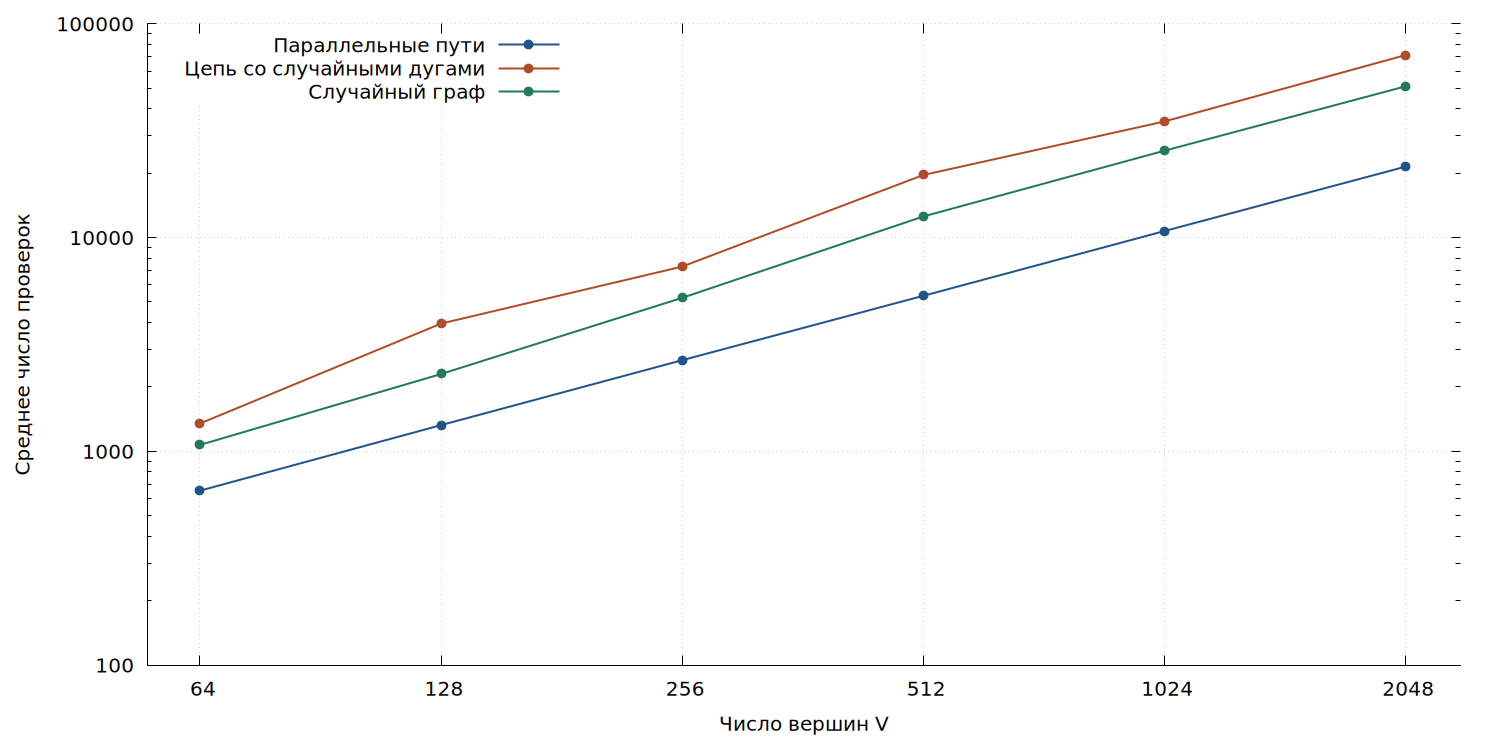
\includegraphics[width=\linewidth]{means.png}
\captionof{figure}{Среднее число проверок при росте $V$. Обе оси логарифмические}
\label{fig:means}
\end{center}

При $V=2048$ и $E=4092$ (рис.~\ref{fig:means}) среднее число проверок у параллельных путей составило \num{21450.8}, у цепи со случайными дугами --- \num{71351.3}, у случайного графа --- \num{50951.2}. Цепь со случайными дугами потребовала в среднем в \num{3.33} раза больше проверок, чем параллельные пути.

При удвоении $V$ среднее увеличивалось в \num{2.00}--\num{2.03} раза у \family{parallel}, в \num{1.78}--\num{2.93} раза у \family{random\_chain} и в \num{2.00}--\num{2.40} раза у \family{random\_graph}. Для \family{parallel} линейный порядок установлен аналитически. У случайных семейств отношение менялось с размером.

Для \family{parallel} значение $\bar C/V$ близко к \num{10.485} и согласуется с формулой~\eqref{eq:parallel-mean}. Во всех сериях отношение $\bar C/(V^2E)$ убывает. При $E=2V-4$ выражение $V^2E$ растёт кубически, поэтому сравнение с ним показывает разницу между измеренными средними и ростом функции из общей верхней оценки. Для случайных семейств наблюдения относятся к исследованным размерам и выбранным правилам генерации~\cite{levitin}.

\clearpage
\subsection{Разброс числа проверок}

\begin{center}
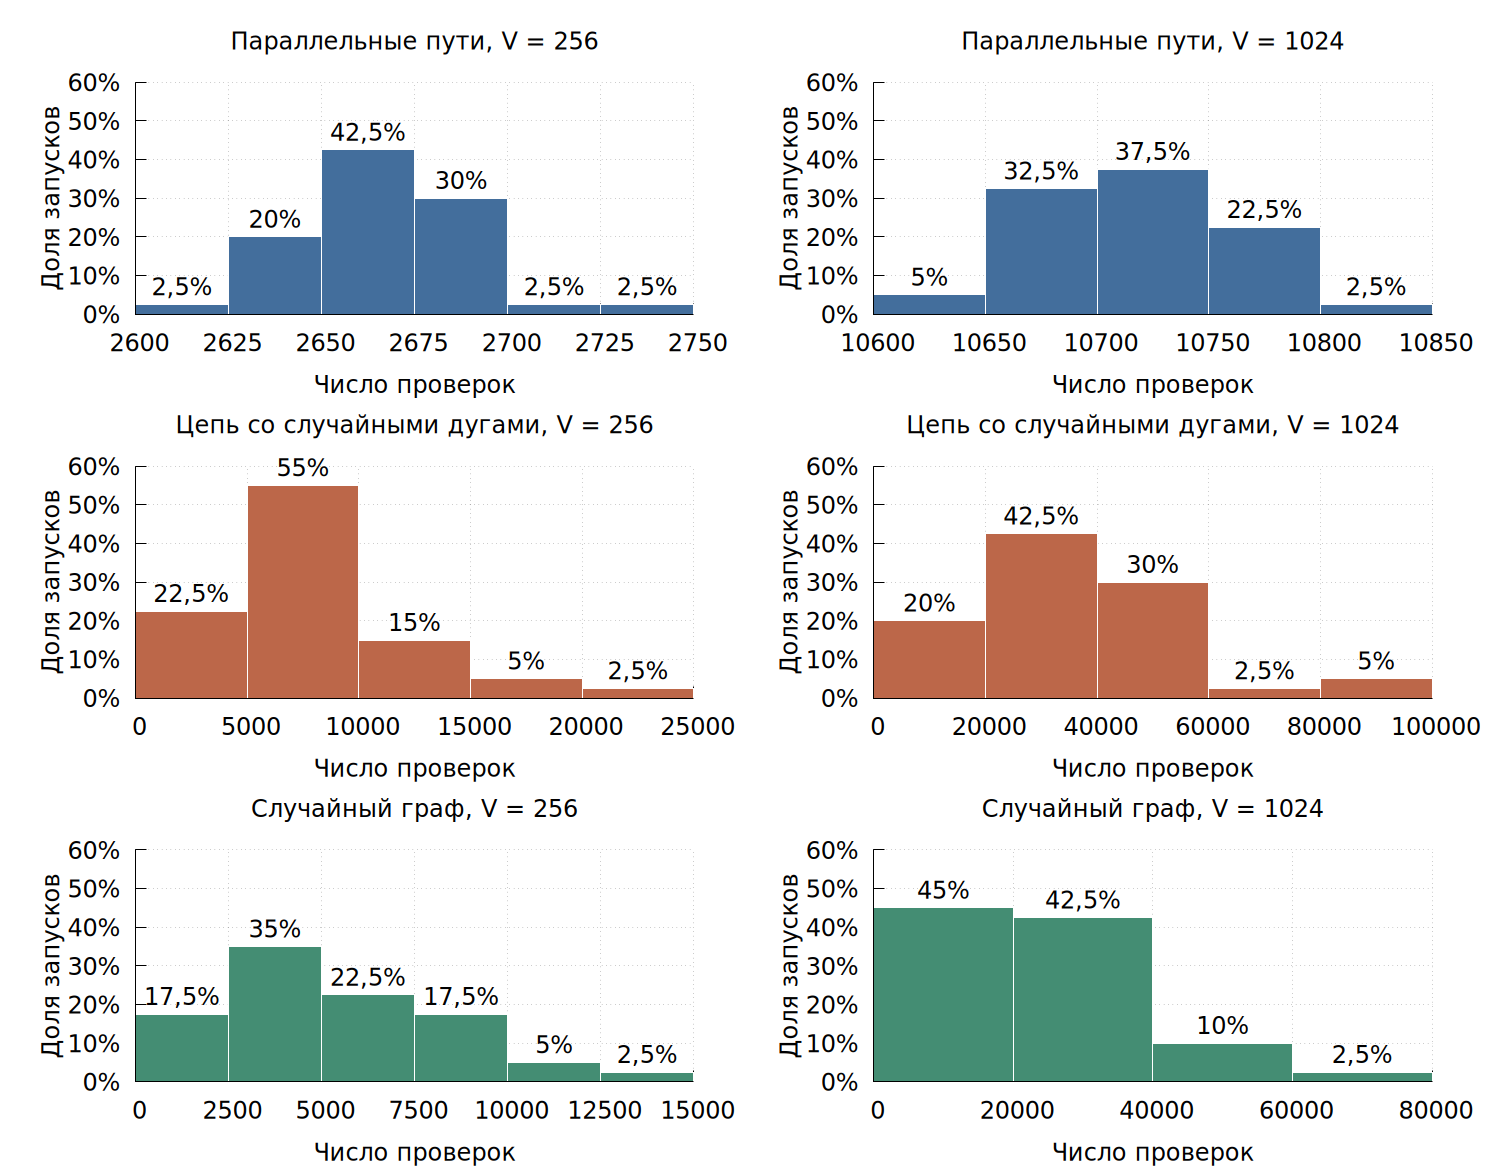
\includegraphics[width=\linewidth]{histograms.png}
\captionof{figure}{Распределение числа проверок для $V=256$ и $V=1024$}
\label{fig:hist}
\end{center}

На рис.~\ref{fig:hist} деления по горизонтали обозначают границы интервалов числа проверок. Высота столбца показывает долю из 40 запусков, попавших в интервал. Например, при $V=1024$ в семействе \family{random\_graph} меньше \num{20000} проверок потребовалось в 18 из 40 запусков (\num{45}\,\%).

Ниже приведено исправленное стандартное отклонение при $V=1024$. В скобках указана его доля от среднего.

\family{parallel} --- \num{43.8} при среднем \num{10719.2} (\num{0.41}\,\%).

\family{random\_chain} --- \num{19642.0} при среднем \num{34906.8} (\num{56.27}\,\%).

\family{random\_graph} --- \num{14421.4} при среднем \num{25470.2} (\num{56.62}\,\%).

В семействе \family{parallel} меняются только ёмкости дуг. В двух случайных семействах между запусками меняются и наборы дуг, и их ёмкости.

\clearpage
\section{Заключение и выводы}

Эксперимент показывает, что при одинаковых $V$ и $E$ и достижимом стоке среднее число проверок и разброс зависят от структуры сети. При $V=2048$ наибольшее среднее у цепи со случайными дугами. При $V=1024$ в обоих случайных семействах стандартное отклонение составляет около \num{56}\,\% среднего. Для параллельных путей линейный рост подтверждается подсчётом проверок.

\section[Характеристики вычислительной среды и оборудования]
  {Характеристики вычислительной\\среды и оборудования}

Linux Mint 22.3 (x86-64), Intel Core i5-12450H, 12 логических процессоров. Компилятор GCC 13.3.0, режим сборки CMake Release, стандарт C++17. Измерялись проверки записей остаточной сети. Графики построены в gnuplot по таблицам \texttt{measurements.csv} и \texttt{summary.csv}.

\renewcommand{\refname}{Список литературы}
\phantomsection
\addcontentsline{toc}{section}{Список литературы}
\begin{thebibliography}{9}
\bibitem{dinic}
Диниц Б. А. Алгоритм решения задачи о максимальном потоке в сети со степенной оценкой // Доклады АН СССР, 1970. Т.~194, №~4. С.~754--757.

\bibitem{sedgewick}
\textenglish{Sedgewick R., Wayne K. Algorithms. 4th ed. Lecture slides, §~6.4 «Maximum Flow». Princeton University.}
\url{https://algs4.cs.princeton.edu/lectures/keynote/64MaxFlow.pdf}

\bibitem{williamson}
\textenglish{Williamson D. P. Lecture Notes on Network Flow. Ithaca, NY: Cornell University, 2007. Technical Report No.~1460. Lecture 11.}

\bibitem{levitin}
\textenglish{Levitin A. Introduction to the Design \& Analysis of Algorithms. 3rd ed. Boston: Pearson, 2012. xxiv, 565 p.}
\end{thebibliography}
\end{document}
